\chapter{Data Analysis}

\section{Efficiencies}
\paragraph{}The high resolution spectrometers are capable of detecting a myriad of particles that track through the detectors. The design of an experimental trigger uses the properties of the individual detectors to capture data of meaningful events. Many accidentals, background, and unwanted events trigger the data acquisition system. The removal of these unwanted events takes place during analysis via software cuts. Restricting the applicable signal from certain detectors through different cuts allows for the rejection of background particles and prevents contamination in the yield extraction. 

\subsection{Particle Identification Efficiency}
\paragraph{} One of the largest sources of contamination for the MARATHON experiment are negatively charged pions. These pions are removed through software cuts made in the total signal from the ten cherenkov PMTs(photomultiplier tubes) and the energy deposited into the blocks of both layers of the calorimeter. Electrons can be identified by their behavior in the spectrometer. High-quality electrons will track through the entire detector stack to deposit most of their energy into the total calorimeter system and creating a large amount of light in the cherenkov. Though this knowledge tight cuts can be used to study the efficiency of the particle identification system. Plotting the signal in the cherenkov versus the energy deposited into both layers of the calorimeter allows for visual representation of the sampling cuts made in the efficiency studies, which can be seen in figure \ref{elesample}. 
\begin{equation}\label{effequ}
\begin{split}
GE_{sample} & = \textrm{Known electron sample from tight cut}  \\
GE_{pass} & = \textrm{$GE_{sample}$ and pass indentification cut} \\
Electron_{eff}  & = \frac{ GE_{pass} } { GE_{sample} } 
\end{split}
\end{equation}
\begin{figure}[]
	\centering
	\textbf{Cherenkov sum versus Total Energy deposited }\par\medskip
	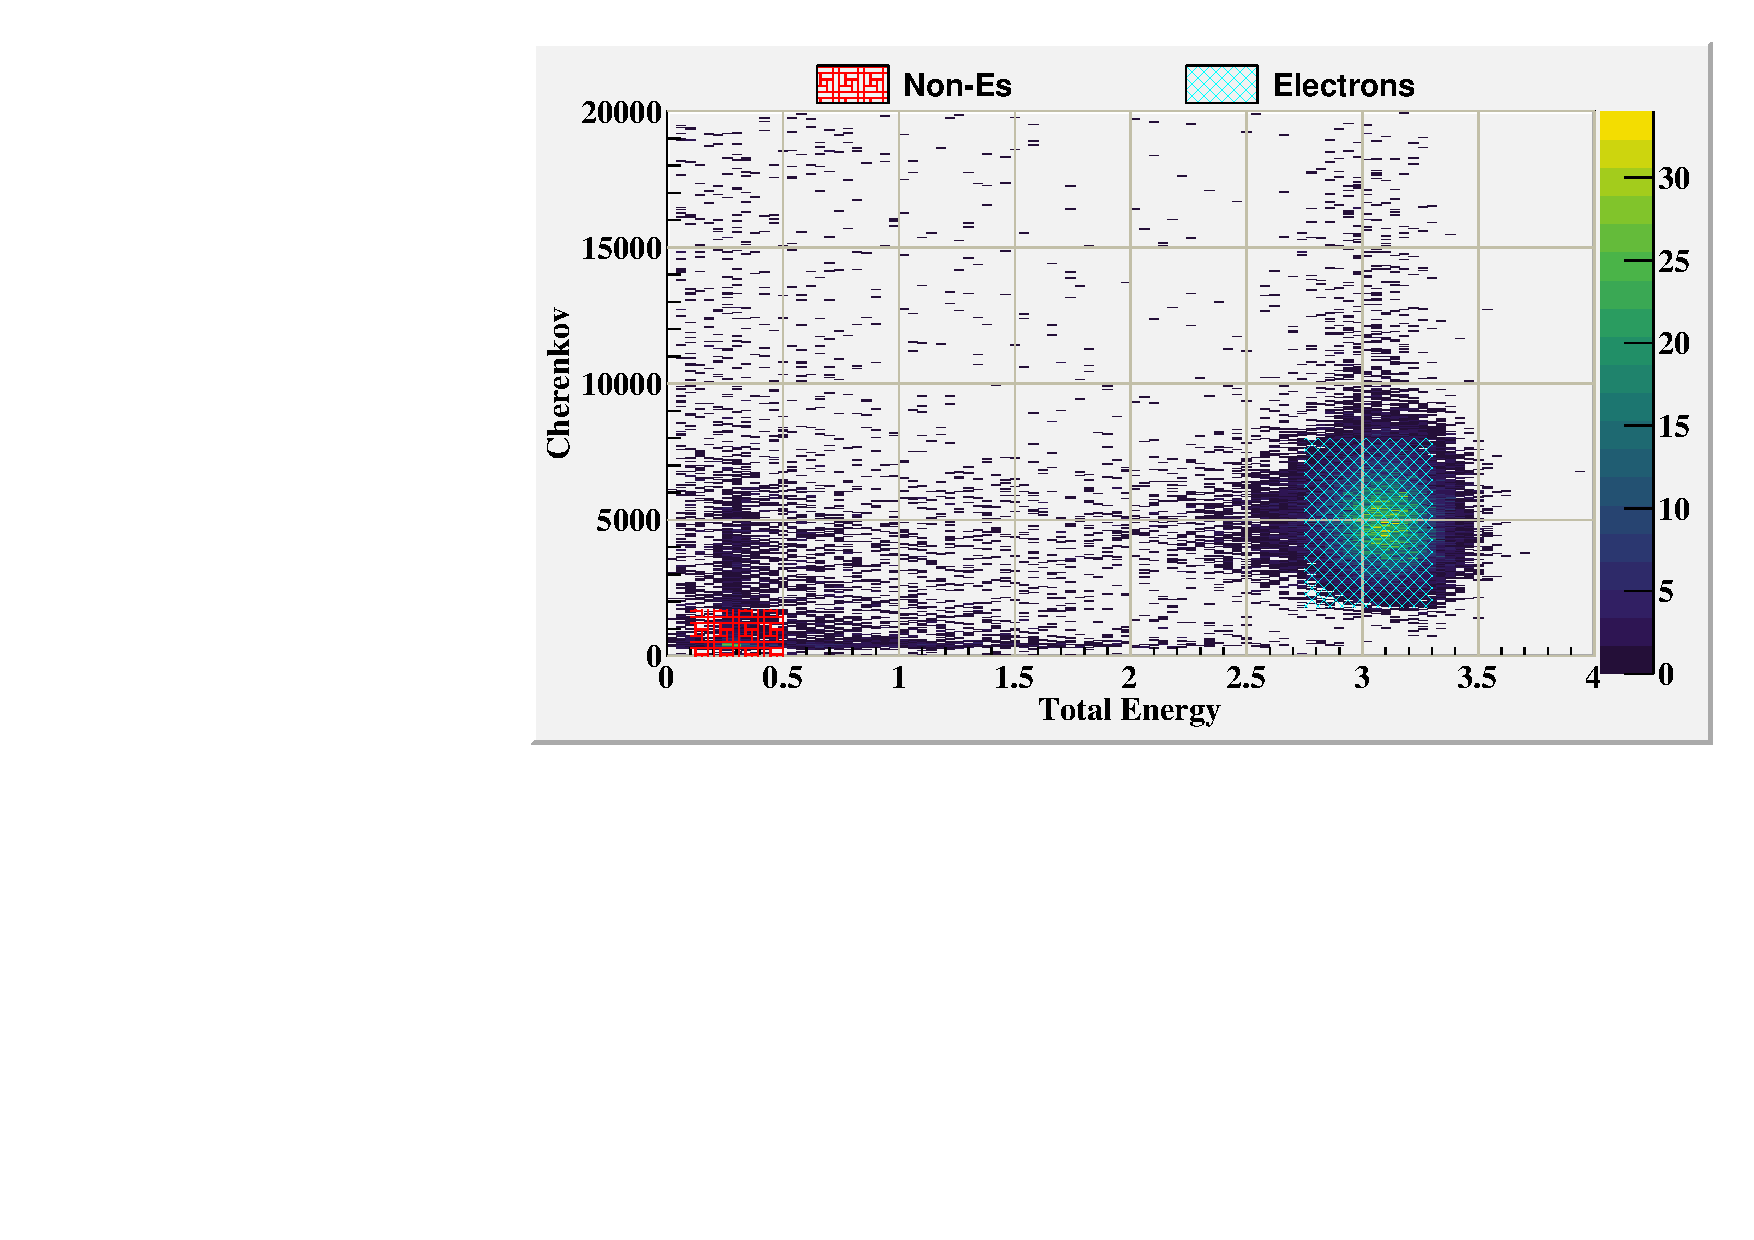
\includegraphics[width=13cm]{PID_2d}
	\caption{Two dimensional plot of the cherenkov sum versus Total Energy deposited, including electron sampling in teal and non-electron sampling in red. }
	\label{elesample}
\end{figure}

\begin{figure}[t]%
	{\centering
		\textbf{Particle ID and efficiency sampling for PID detectors }\par\medskip}
	\centering
	\subfloat[]{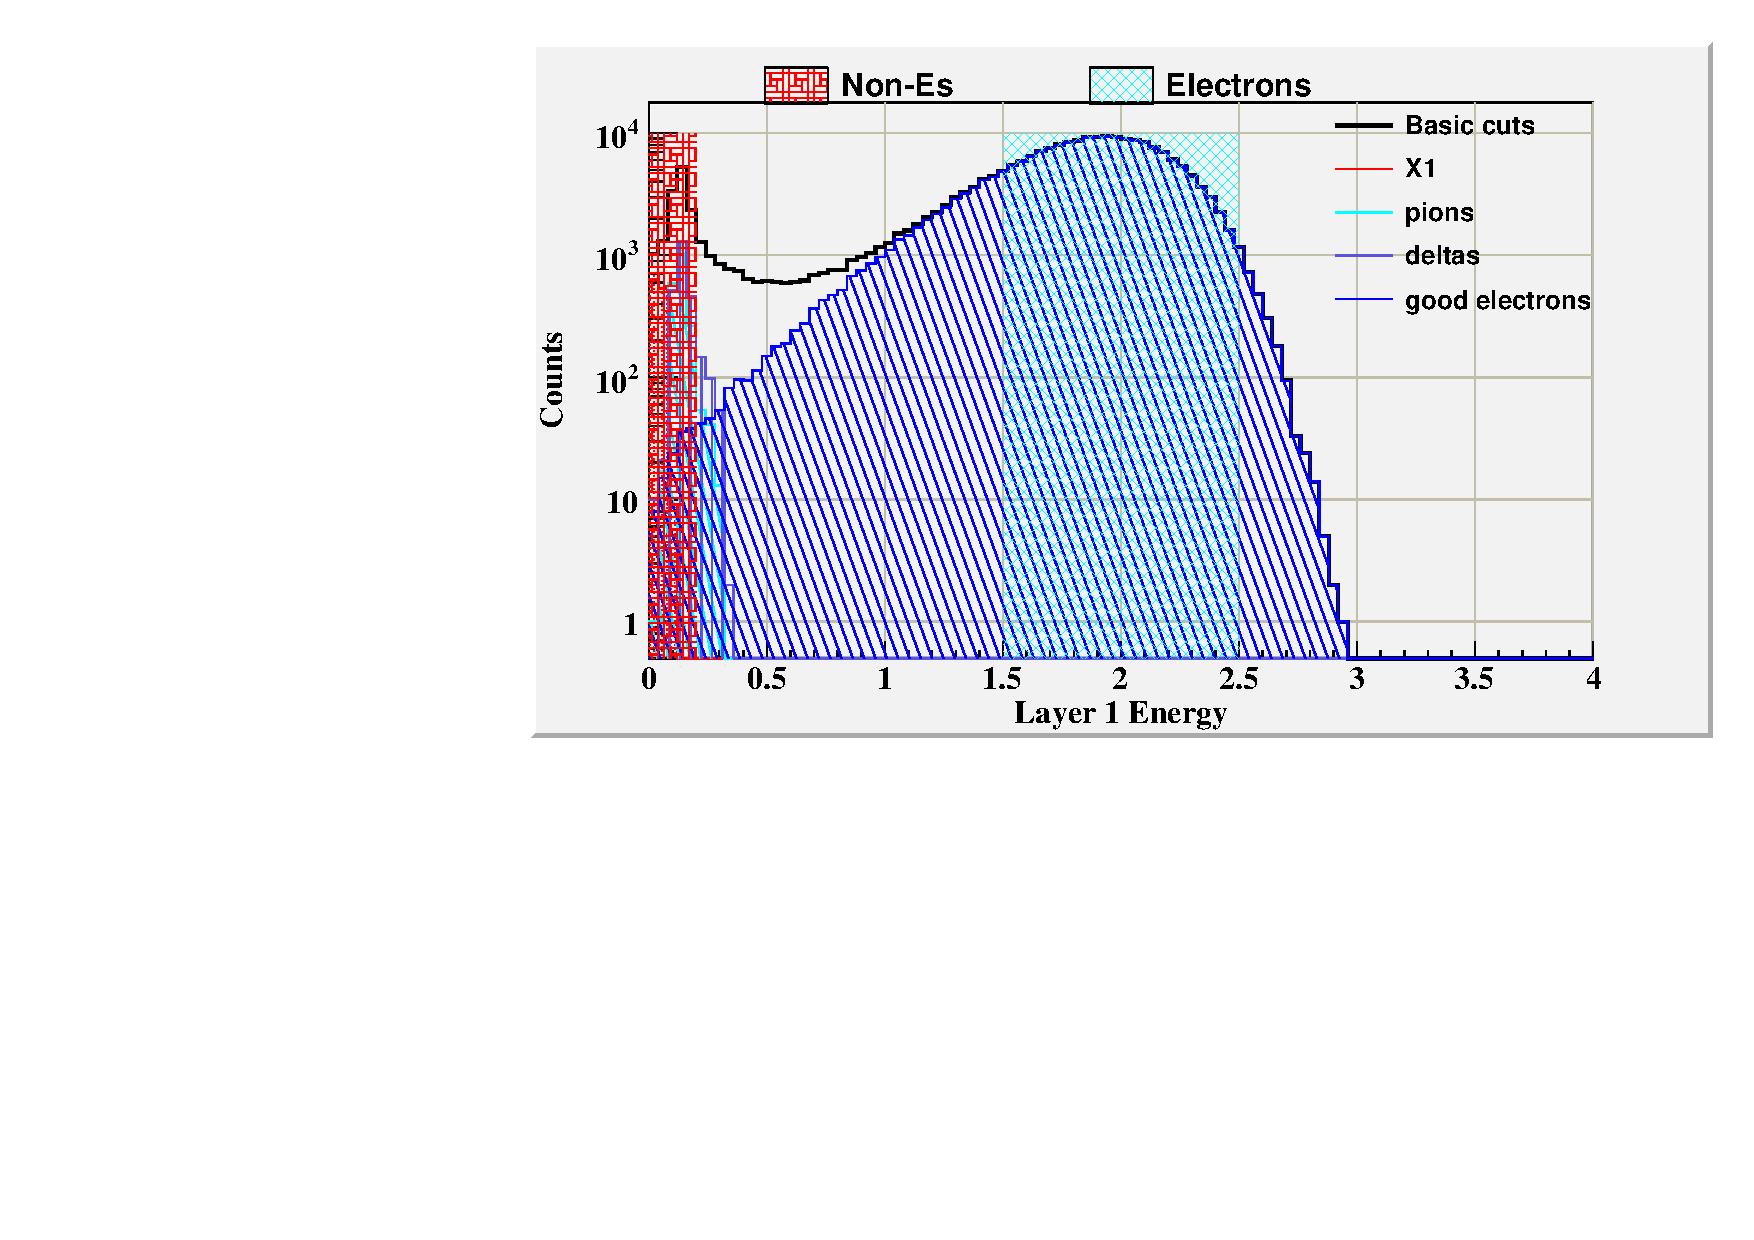
\includegraphics[width=0.5\textwidth,height=4.5cm]{Lprl1}\label{samA}}%
	\subfloat[]{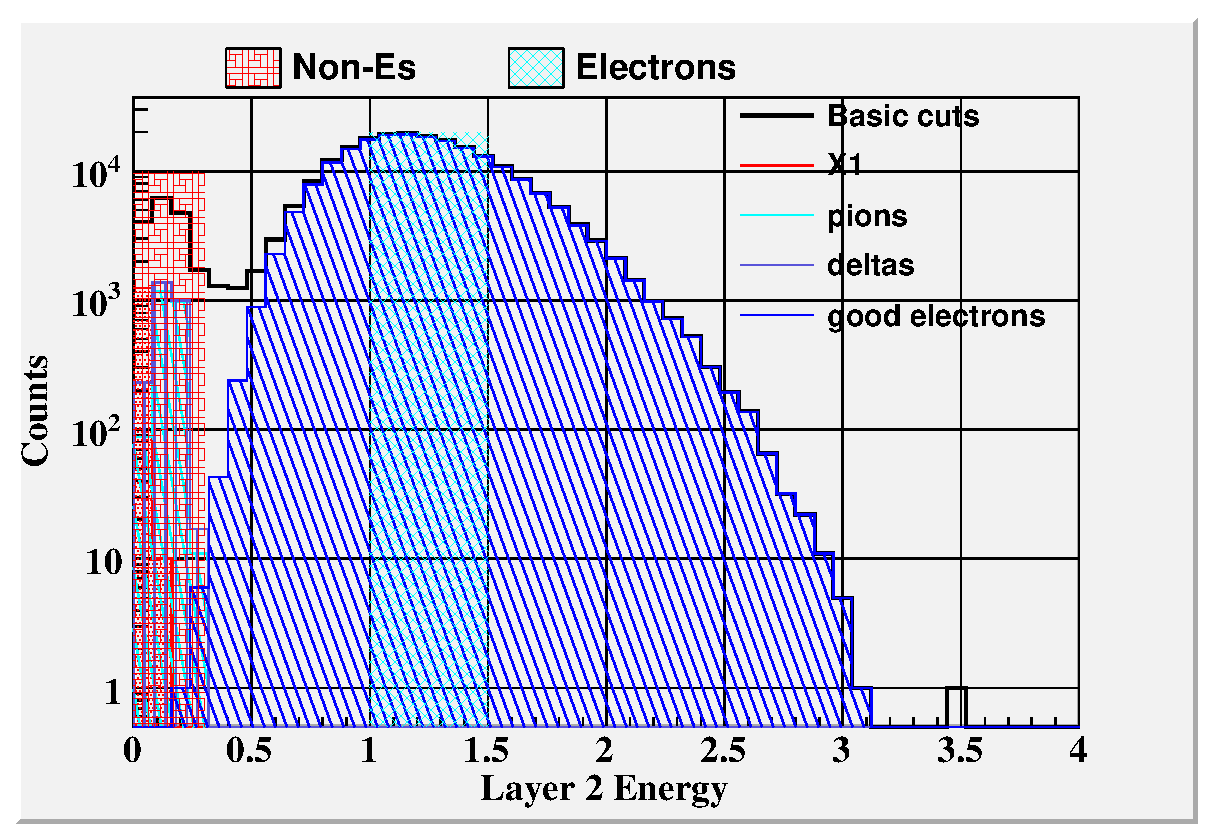
\includegraphics[width=0.5\textwidth,height=4.5cm]{Lprl2}\label{samB}}\\
	\subfloat[]{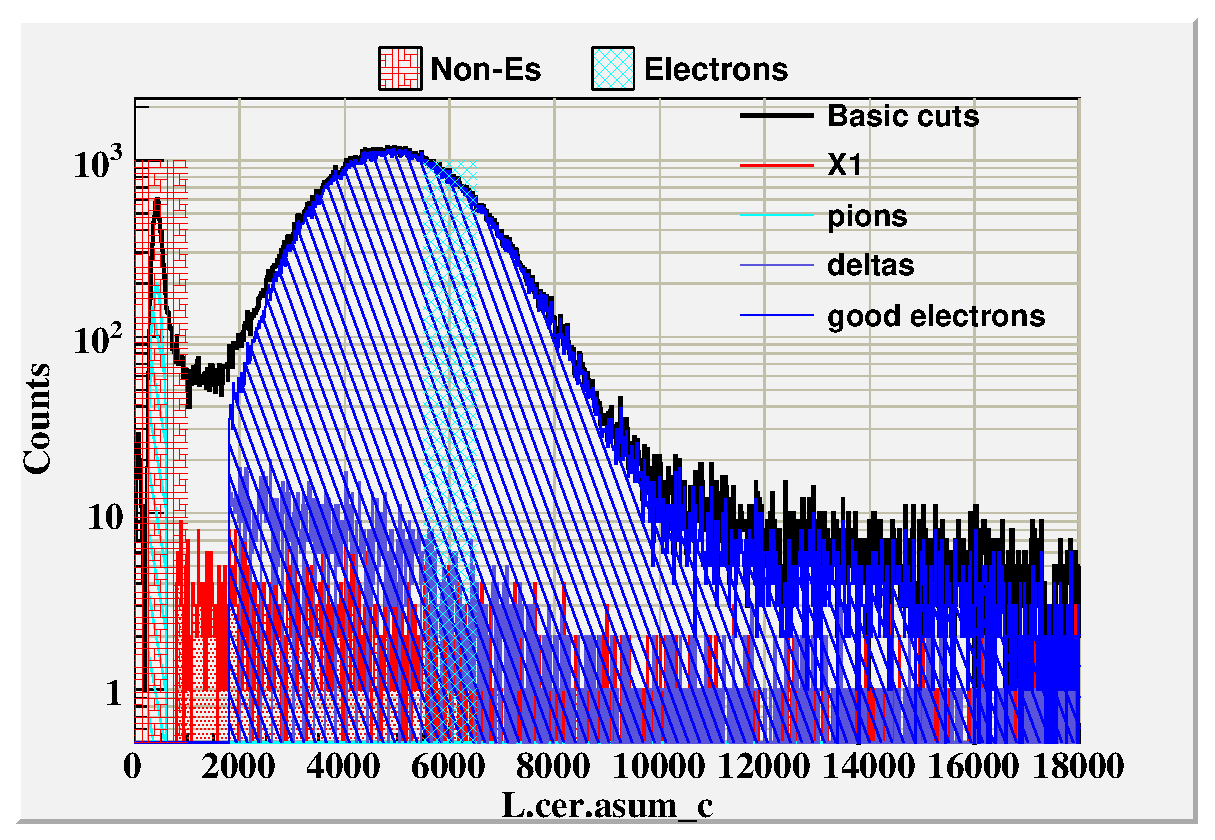
\includegraphics[width=0.95\textwidth,height=3.85cm]{Lcerasum}\label{samC}}%
	\caption{Electrons and other back ground particles identified via cuts in the total calorimeter and the gas cherenkov shown in the individual layers of the calorimeters and the cherenkov. Sampling cuts for Electrons in teal and Non-Electrons in red.}%
	\label{sampling}%
\end{figure}


\paragraph{}The efficiencies of the spectrometer's particle identification(PID) detectors were determined by using the first calorimeter layer, the second calorimeter layer, and the cherenkov to provide samples of good electrons and other particles. The PID efficiency of the individual detectors was determined using equation \ref{effequ}. The good electron sample for calculating the efficiency of the single detector was defined by sampling through the other two detectors. Sampling through the two layers of the calorimeter is shown in figure \ref{samA} for the first layer of the calorimeter and \ref{samB} for the second layer. The cherenkov good electron sample is shown in figure \ref{samC}. The electron sample from the cherenkov is contaminated by delta particles and a combination of unknown particles. These unidentified background particles are known to be relativistic due to the amount of light seen in the cherenkov. However, the events do not deposit enough energy into the calorimeter system to be considered as a good electron that scatter from our target through the detector. Using sampling in one layer of the calorimeter and the cherenkov, these unwanted low energy particles are rejected from sampling for efficiency calculations. The electron selection PID efficency for the three PID detectors was determine at each kinematic setting to be approximately 98$\%$ . The efficiency was determined to be independent of the kinematic setting. Only small fluctuations were seen during the study, these small changes are due to decrease in statics, and all of the results fall within statical uncertainty of being independent of kinematic setting. The non-electron suppression efficiency was determine as part of this PID efficiency study to ascertain how many back ground particles leak into our sample of good electrons after cuts our made. The suppression efficiency of the cherenkov suffered due to the contamination of the relativistic low energy particles. Combining the two calorimeter detectors with the cherenkov increased the overall suppression efficiency for the spectrometer to 99.9$\%$ over the entire kinematic range of the MARATHON experiment. 

\begin{figure}
	{\centering
		\textbf{PID efficency for each detector for all kinematics. }\par\medskip}
	\centering
	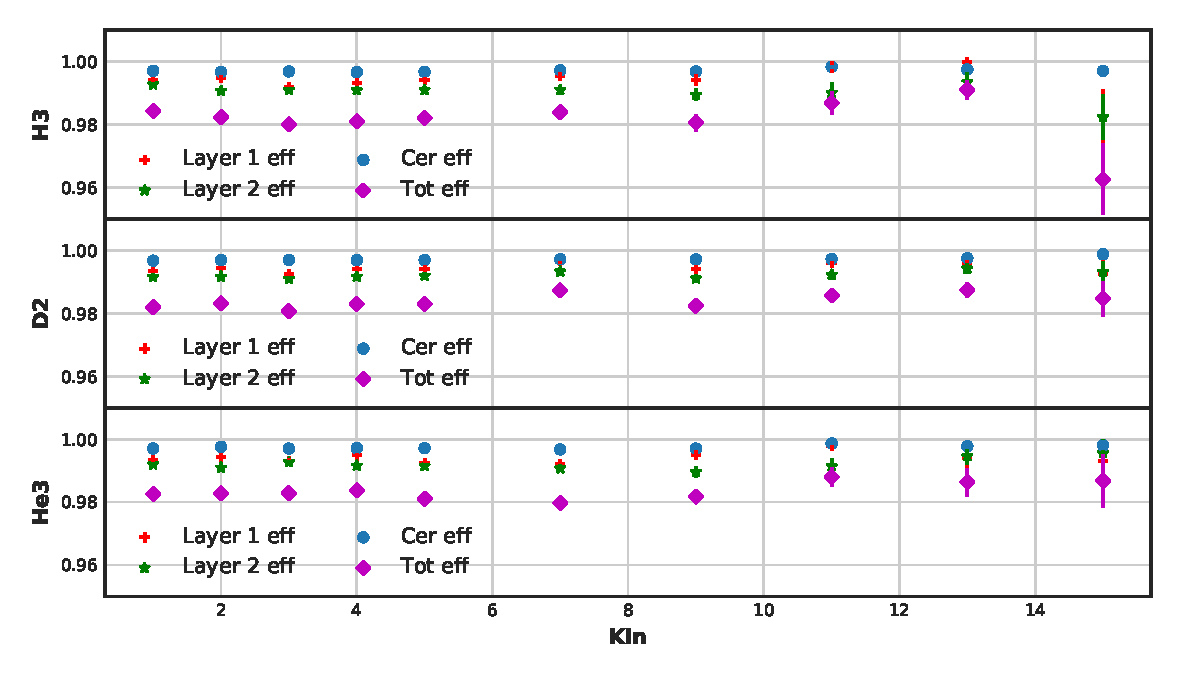
\includegraphics[width=12cm]{PID_allkin_alltgt}
	\caption{The PID efficiency for the cherenkov and both layers of the calorimeter,including the overall total PID efficiency for each of the gas targets at all of the kinematics.}
\end{figure}

\subsection[]{Trigger Efficiency} 



